%!TEX root = thesis.tex
%=============================================================================


\section{Dataset Evaluation}

In this section, evaluation of the proposed pipeline and an existing solution on a dataset will be presented.
The goal of this evaluation is to take a closer look on the performance of the proposed pipeline with the explicit focus on computational cost as well as time needed for recognizing speech.

Based on the additional features the proposed pipeline introduces, most prominently synchronization of speech results and the modular nature of the pipeline, as presented in chapters TODO, we expect the proposed pipeline to consume more CPU power as well as taking longer to compute results in comparison to the existing solution.
To further examine the cost, we will in particular inspect the cost different additional components will add to the pipeline, to determine the scaling of the proposed pipeline.

We will lastly discuss if this additional cost makes using the pipeline unsuitable for real world applications or if the benefits overweight these costs.

\subsubsection{Dataset}

The dataset used for this evaluation consists of 1723 samples with length between a half and fourteen seconds.
It incorporates 12 speakers (male and female) speaking 24 phrases. 
Individual samples were recorded using two microphones, one omni directional and one cardioid.
They were recorded in two rooms, some of them with noise, others without.

To more easily feed all samples into the existing solution, the wav files containing the samples were concatenated into one big wav file, with three seconds of silence added in between the individual samples, to distinguish the samples from one another and make it possible for the used speech recognizer to separate them.
This simplifies matching the recorded speech recognition results with the actual utterances.
The proposed pipeline was fed each sample individually, but three seconds of silence were similarly inserted into the audio.

The playtime of the complete dataset including the silence amounted to nearly two hours and fifty minutes.

\subsubsection{Setup}

Two slightly different setups were used for the various configurations of the proposed pipeline on the one hand and the existing solution on the other hand, due to differences in acquiring audio data.
What the have in common is that all pipeline were tested on the same computer, a Thinkpad Carbon X1 Gen with a Intel(R) Core(TM) i7-7500U, to ensure equality in CPU performance.

All were comprised of equivalent components. 
If not otherwise stated, all variations of the proposed pipeline used the exact same components with identical configurations (safe for some minor details, e.g. a modified path for the audio between the wav player, dummy node and VAD in the elongated version of the proposed pipeline, see figure \ref{pic:eval_p2_diag} and \ref{pic:eval_p4_diag}).

The existing pipeline's PocketSphinxAdapter internally incorporates a VAD, which was reimplemented and used as the VAD of the proposed pipelines.
It uses PocketSphinx for speech recognition, as does the speech recognizer used in the proposed pipeline. 
Both PocketSphinx instances use the same speech models, dictionary and grammar.

In both cases two small scripts were used to record the components CPU usage as well as speech recognition results and timings.
CPU usage was universally recorded using the python library psutil and its cpu\_times functionality.
However, psutils reliability can be called into question, as it seems not to take into account modern CPU's capability to increase or decrease their clock speed, depending on load.
As such, the recorded CPU costs should rather be taken as rough estimates and not as exact measurements.
We included this data points despite their supposed inaccuracy because apart from the last tested pipeline, all pipelines did not produce enough load on the CPU to cause it to increase its clock speed.
This is supported by fact that identical components across various pipelines produce nearly identical CPU loads.

Speech recognition results were recorded by a ROS node which collected ROS messages published by the proposed pipelines orchestrator respectively the PocketSphinxAdapter.

\subsubsection{Result Recording}

The times needed to calculate results were recorded in two different ways.
Due to the fact that the proposed pipeline annotates its results with the time the audio was recorded, it is rather simple to calculate the time needed for recognition.
One can just subtract the time when the analyzed audio signal ended from the time the synchronized result was received by the recording component an thus get the absolute time needed for recognition.

As such the method of feeding audio into the proposed pipeline does not matter as long as the time stamps of the audio are correct, so instead of grabbing the audio via a microphone we used a wav-file player to feed the dataset directly into the pipeline.

The existing solution however was in need of a small workaround to work on audio files rather then audio directly grabbed by a real microphone.
A virtual microphone was needed to feed the dataset into the PocketSphinxAdapter.
This virtual microphone provided access to a wav file containing the dataset. 
As information about singular utterances inside the dataset could not be propagated through ALSA and the PocketSphinxAdapter, we recorded a time stamp with the start of feeding the wav file into the virtual microphone and thus in turn into the PocketSphinxAdapter.
Speech recognitions results were then recorded along time stamps acquired when these results were received in the dedicated ROS node.
Supplementary, the while concatenating the dataset into the singular wav file, we created annotations to keep track of when each sample ended.

By combining the information provided by these annotations, the time stamp created during the start of feeding the wav file and the time stamps recorded when recording the speech recognition results, the absolute time needed by this solution could be computed.

In any case, speech recognition results and timings were recorded as raw data and written to files.
Afterwards, these raw results could be processed and evaluated with the help of further scripts.


\begin{figure}[ht]
	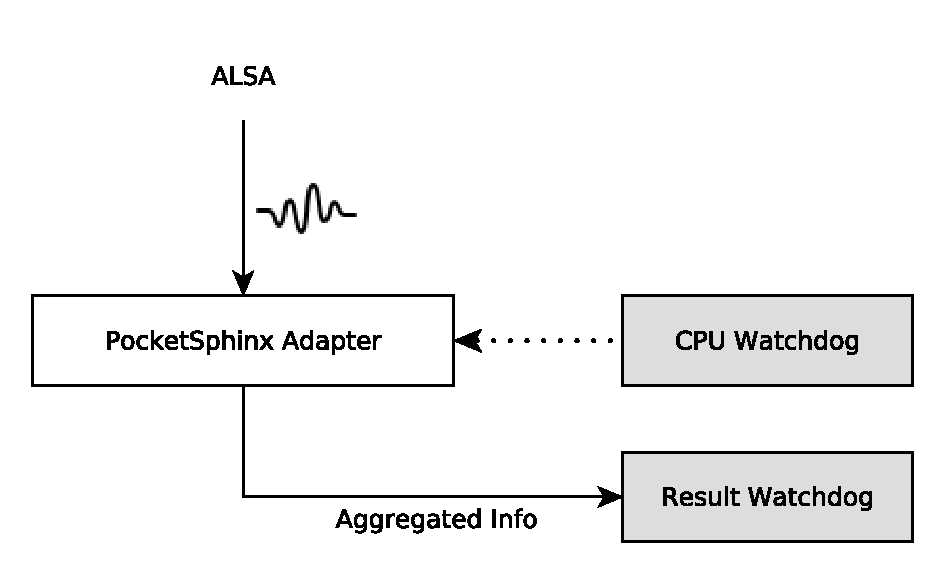
\includegraphics[width=0.66\textwidth]{diagrams/eval_pipeline_1.pdf}
	\caption{Test scenario for existing pipeline}
	\label{pic:eval_p1_diag}
\end{figure}

\begin{figure}[ht]	
	\centering
	\subfloat[Scenario for baseline of proposed pipeline]{
		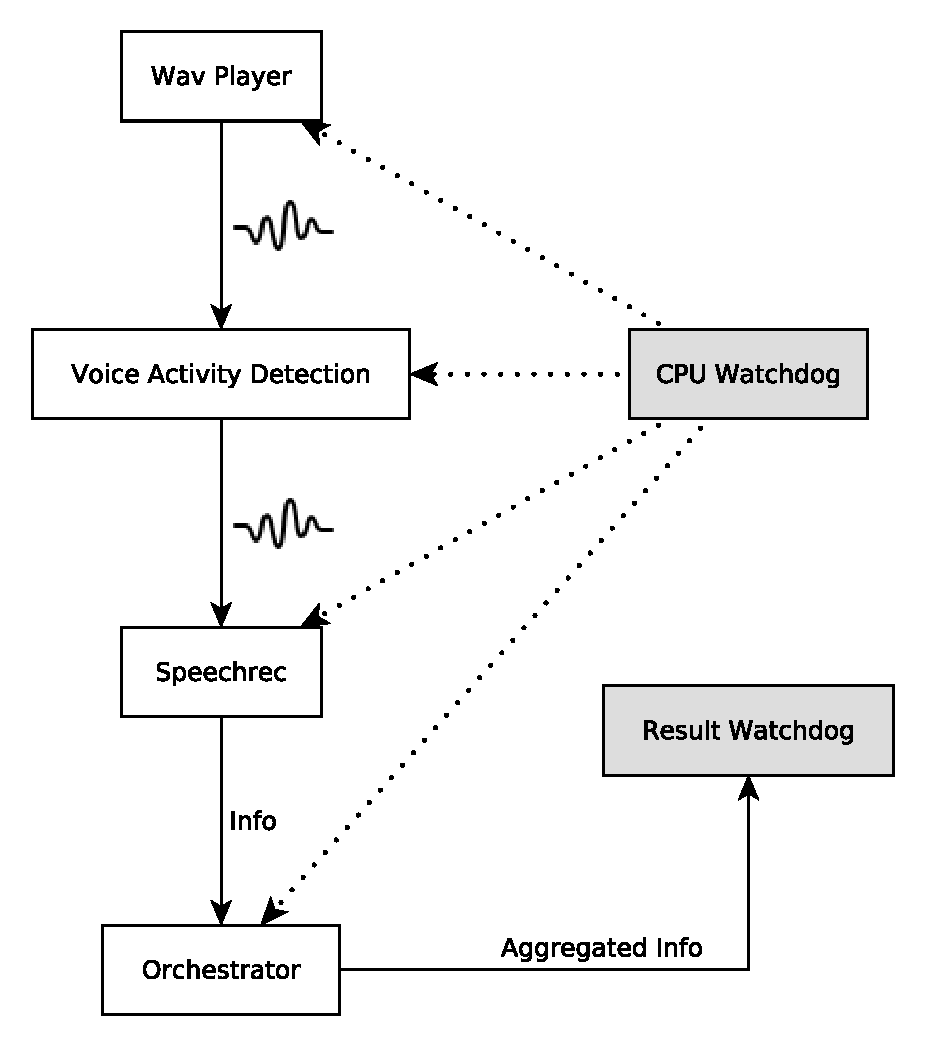
\includegraphics[width=0.5\textwidth]{diagrams/eval_pipeline_2.pdf}
		\label{pic:eval_p2_diag}
	}
	\subfloat[Scenario for elongated baseline of proposed pipeline]{
		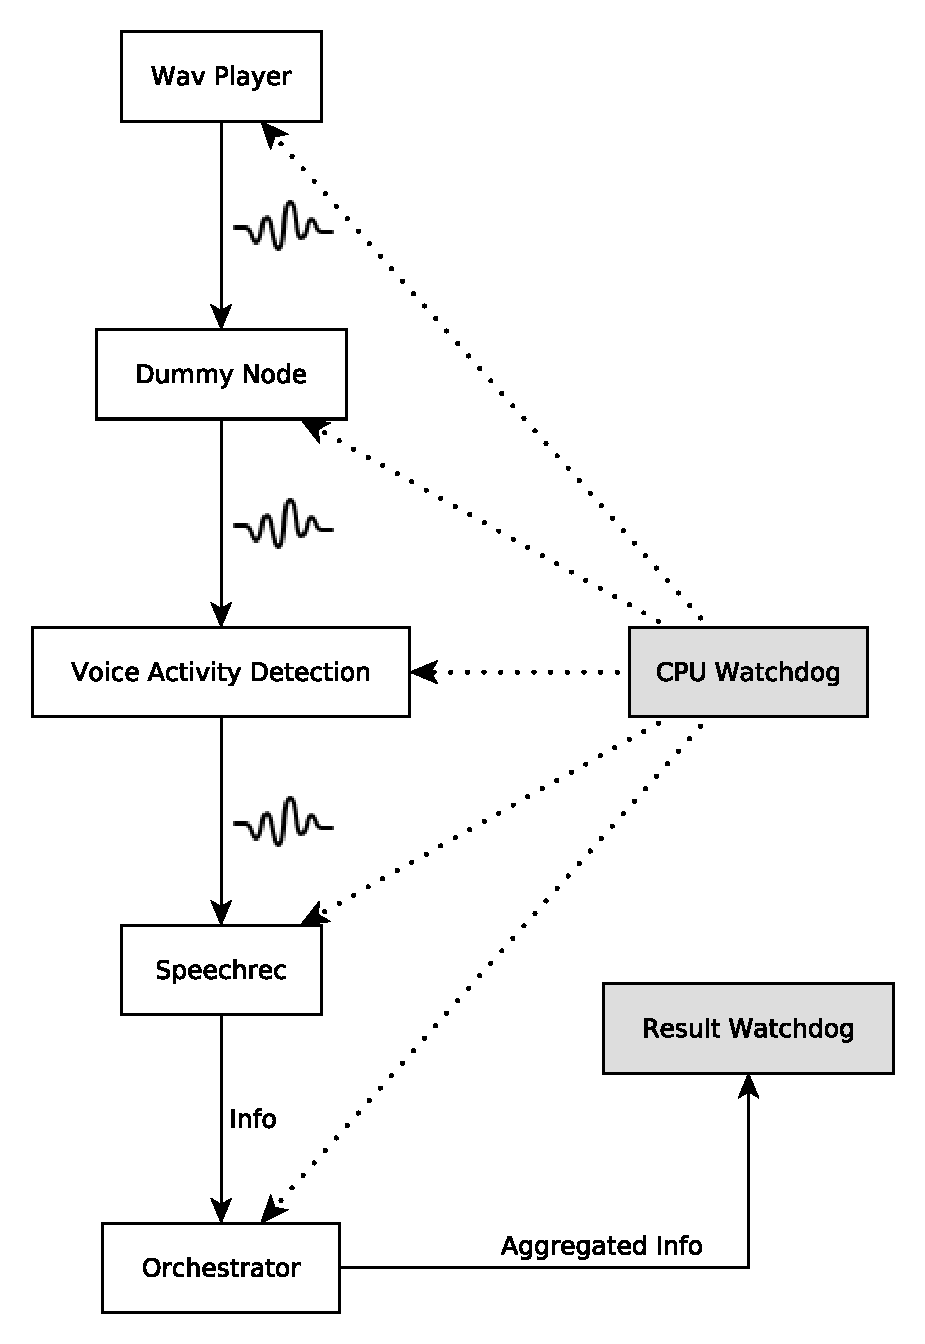
\includegraphics[width=0.5\textwidth]{diagrams/eval_pipeline_4.pdf}
		\label{pic:eval_p4_diag}
	}
	
	\caption{Test scenarios for proposed pipeline}
	\label{pic:eval_p2_4_diag}
\end{figure}


\begin{figure}[ht]	
	\centering
	\subfloat[Test scenario for widened baseline of proposed pipeline]{
		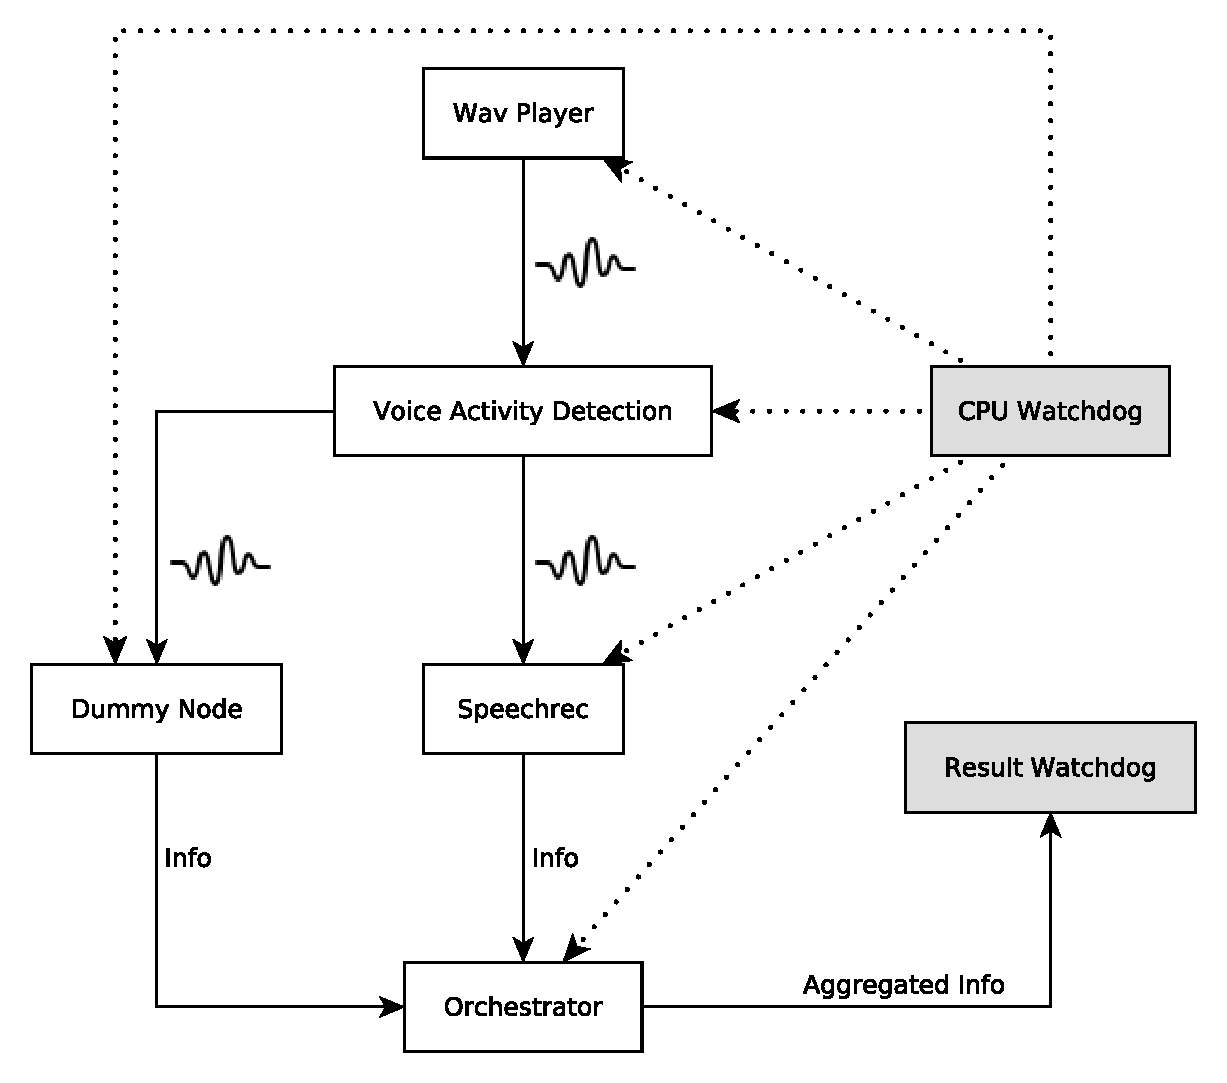
\includegraphics[height=0.4\textwidth]{diagrams/eval_pipeline_3.pdf}
		\label{pic:eval_p3_diag}
	}
	\subfloat[Test scenario for elongated baseline of proposed pipeline]{
		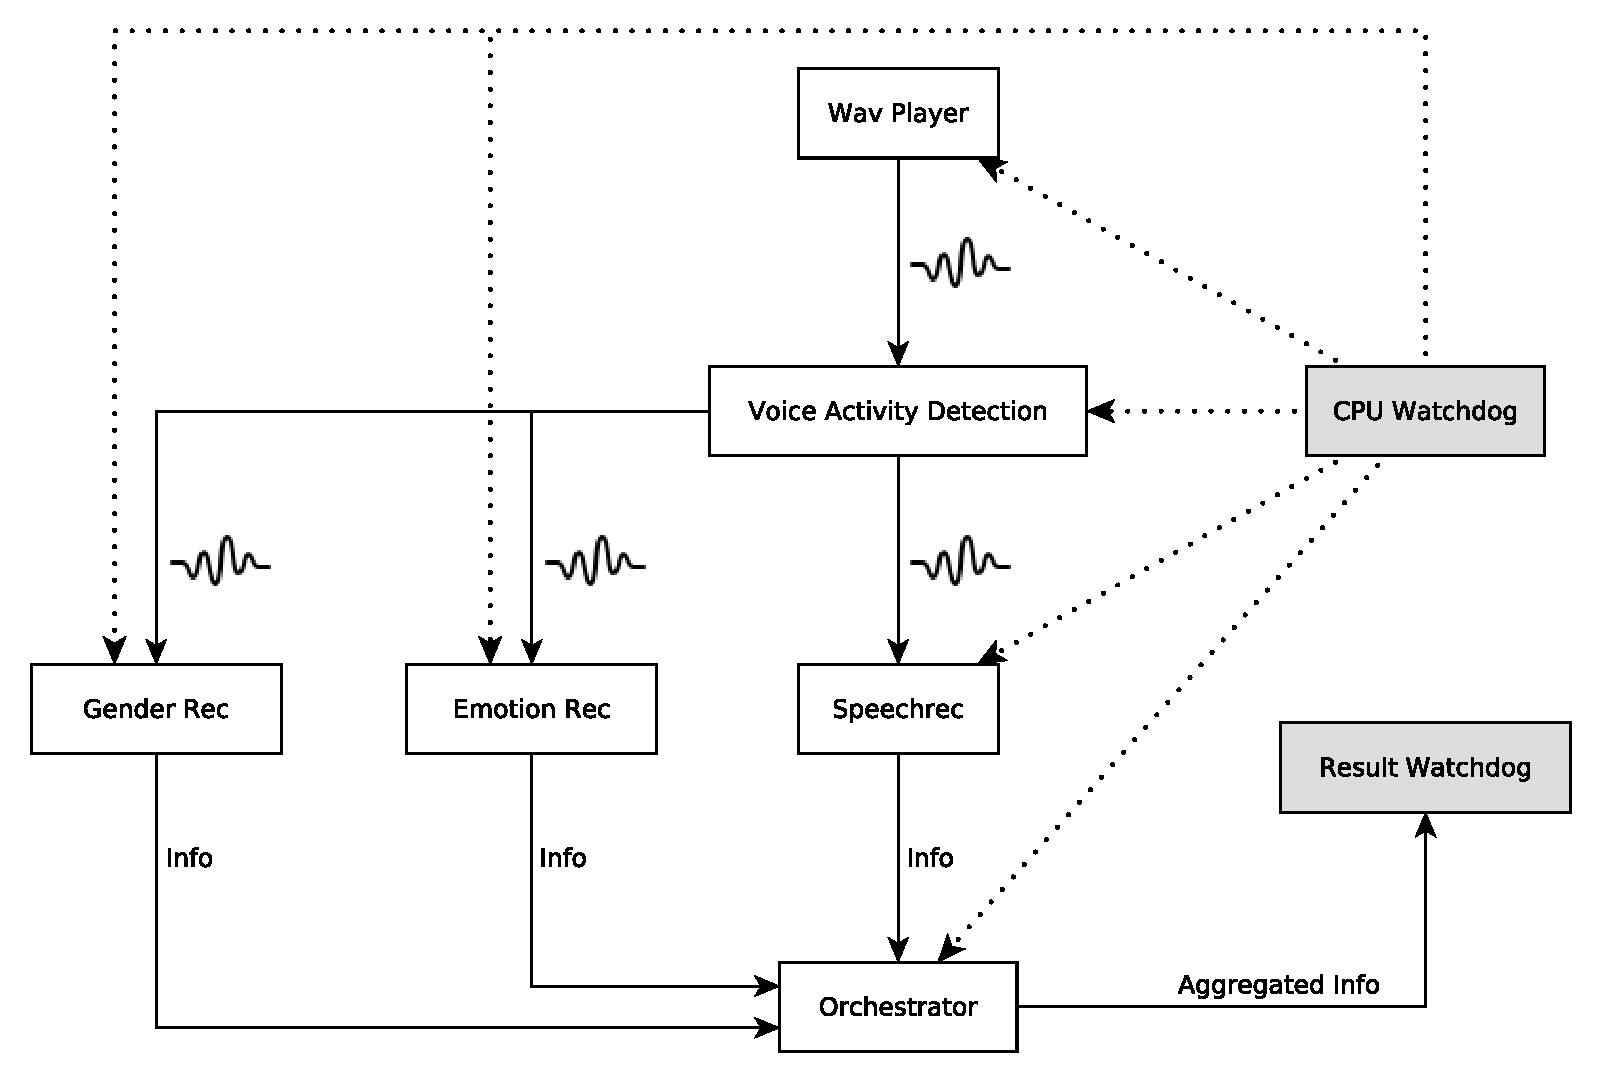
\includegraphics[height=0.4\textwidth]{diagrams/eval_pipeline_5.pdf}
		\label{pic:eval_p5_diag}
	}
	
	\caption{Test scenarios for proposed pipeline}
	\label{pic:eval_p3_5_diag}
\end{figure}

\begin{figure}[ht]
	\begin{tabular}{ | l | p{0.3\textwidth} | p{0.3\textwidth} | p{0.3\textwidth} |}
		\hline
		Pipeline & Correctly recognized sentences & Absolute time till result (in seconds) & CPU time (in CPU seconds) \\ \hline
		Existing & 77.19\% & 1.5596 &  247.44 \\ \hline
		Proposed & 99.77\% & 1.0141 & 1209.3 \\ \hline
		Elongated & 99.77\% & 1.0394 & 1399.63 \\ \hline
		Widened & 99.65\% & 1.0899 & 1665.66 \\ \hline
		Realistic & 99.48\% & 1.7799 & 37517.13 \\ \hline
	\end{tabular}
	\caption{Results of the pipelines in comparison}
	\label{table:eval_dataset_results}
\end{figure}


\subsection{Existing Solution}

Little description:
The existing solution consists only of the PocketSphinxAdapter (PSA), see figure \ref{pic:eval_p1_diag}.
The PSA grabs audio from a microphone using ALSA, filters the audio using an integrated voice activity detection and finally uses, as its name suggests, PocketSphinx to recognize speech.
Recognition results are then communicated via ROS.

Goal: provide a baseline

What can be seen: 

\subsection{Baseline for proposed Pipeline}
Little description:
This configuration of the proposed pipeline is intended to reassemble the PSA as closely as possible.
As seen in figure \ref{pic:eval_p2_diag}, it consists of a voice activity detection, a speech recognizer (using PocketSphinx), the Orchestrator and a Wav file player to feed audio into the pipeline.
Recognition results are gathered by the Orchestrator and then communicated via ROS.

Goal: get additional cost the pipeline itself generates against the existing solution

What can be seen: 

If one compares the results of the pipelines in figure \ref{table:eval_dataset_results}, 
- results for the proposed pipeline are all virtually identical, 


\subsection{Elongated baseline of proposed Pipeline}
This configuration of the proposed pipeline is nearly identical to its baseline, but incorporates a dummy component to evaluate how much overhead in time and CPU cost an additional processing step produces.
As indicated in figure \ref{pic:eval_p4_diag} and by its name, the dummy node does neither alter nor compute information on the audio data it received, but instead just relays it from the WAV player to the VAD.

If one compares the results of the proposed and elongated pipeline in figure \ref{table:eval_dataset_results}, a slight increase in absolute time per recognition can be seen, as well as a moderate increase in CPU cost.
The slight increase of 15ms in absolute recognition time can be expected 
The increase in CPU cost is virtually completely due to the additional dummy component present in this pipeline. 
Its CPU cost lies a little below the cost of the VAD, which utilizes a computationally very inexpensive algorithm to segment the audio, so it presents a compelling baseline for TODO



What can be seen: overhead cost of adding component is rather small, especially in absolute time needed (2.5 ms), thus negligible

\subsection{Widened baseline of proposed Pipeline}
This configuration of the proposed pipeline is nearly identical to its baseline, but incorporates a dummy component to evaluate how much overhead in time and CPU cost an additional information provider produces.



Goal: get overhead cost of a parallel component

What can be seen: 

\subsection{Realistic version of proposed Pipeline}


Goal: 

What can be seen: 


\section{Discussion}

However, it is good to keep in mind that PocketSphinx was designed years ago to work on mobile devices of that time, so it is one of the computational most inexpensive speech recognizers still used. 
More modern speech recognizers can generally be divided into offline and cloud services.

Cloud based speech recognizers, such as Google or Microsoft speech to text services produce varying degrees of latency, as audio must first be streamed to distant datacenters before it can be processed and the results can be sent back.
Depending on the available internet connection and the time spend analyzing the audio, these approaches typically take at least as long as fast offline approaches.

Modern offline approaches mostly focus on deep learning at the time of writing. 
As such they often use elaborate neural networks which can only be run on graphics cards in a timely manner and are computationally exceptionally costly.

The results of the last version of the proposed pipeline reflect this.
Both the gender and emotion recognizer used in the pipeline use rather simple, but nevertheless computationally costly neural networks.
Still they exceed the cost of all other pipelines by more than a factor of 20.

Based on this and the fact that all components of the proposed pipeline can easily swapped out, the actual resource cost the components themselves introduce are mostly uninteresting, as each component could easily be replaced.